\section{Research -- Phase I}
\label{sec:research}

The goal of the overall system is to support exploration of aggregated data. 
To achieve this goal, we will leverage our current IoT infrastructure
to implement privacy-preserving data aggregation techniques from the
differential privacy literature.
The data processing, computation, and aggregation occur in the
back-end where the data reside.
The processed data sent to the front-end visualization system will
contain aggregated data for clients and stakeholders to interact with.

During Phase~I, our focus will be on addressing the following three
research questions.
\begin{enumerate}
\item[\textbf{R1:}] Can we effectively reduce differential privacy theory to practice,
balancing the conflicting concerns of privacy budget and data utility, in
the context of the agricultural marketplace?
\item[\textbf{R2:}] What incentives are required for farmers to be willing
to share their data?
\item[\textbf{R3:}] Can we effectively communicate aggregated time series data,
with the inherent uncertainty imposed by differential privacy, to end users?
\end{enumerate}

We anticipate addressing the first question through empirical evaluation,
exercising one (or more) privacy-preservation algorithms across agricultural
IoT data and assessing the resulting output in the privacy
versus utility tradeoff space.  We will address the second and third questions
by exploring several incentive mechanisms and
visualization approaches and assessing their effectiveness
through user studies.\footnote{For all user studies, we will seek the
appropriate human subjects approvals through the IRB at Washington
Univ.~in St.~Louis.}

\subsection{R1: Data Aggregation and Privacy Preservation}
\label{sec:da}

We are interested in assessing our ability to reduce differential
privacy theory into effective practice, and our approach to achieving
that goal is empirical evaluation.  That implies collecting data,
performing experiments, and evaluating the experimental outcomes.
We will describe each of these in turn.

\paragraph{Data Sources}
The Feed-Link system currently provides cloud-based access to
agricultural sensor data owned by the individual farmer.
BECS is the trusted curator of that data, responsible for its security,
integrity, and availability.  To provide experimental
data for the proposed privacy preservation research, in
consultation with GSI (our private-label partners), we will query 
current customers and ask permission to use historical data from their
farms.  There are a number of customers that regularly assist
us in evaluating new products, etc., at their farm, such that we anticipate
no difficulty in achieving data access from real-world installations.

%In addition to customer data, BECS maintains a wet wall test facility in
%its plant (see Facilities, Equipment and Other Resources) that has multiple
%instances of water treatment control and monitoring equipment installed.
%Data are available from this facility going back several years.

\paragraph{Experiments}
Our initial empirical investigation will focus on the approaches
described by Fan and Xiong~\cite{fx12,fx14}, utilizing their
FAST (Filtering and Adaptive Sampling for differentially private
Time-series monitoring) framework. Individual experiments will have
as inputs:
\begin{itemize}
\item an example aggregated time series data set,
\item settings for the privacy budget
(i.e., values of $\epsilon$ and $\delta$),
\item parameter values for FAST (i.e., see Table~1 of \cite{fx14}), and
\item prediction/correction filter for FAST (Kalman vs.~Monte Carlo)
\end{itemize}
and will provide an output time series that is differentially private.
Using any number of techniques (e.g., relative error, correlation analysis), 
we can then compare the input (non-private) time series to the output
time series.
We will use $2^k$ factorial experimental design~\cite{Jain91}
to reduce the overall empirical search space to manageable levels,
adding experiments as needed to fill in portions of the space that
appear interesting.

Of course, the real world is never as simple as implied by the previous
paragraph.  E.g., $\delta= 0$ in the published version of FAST.
Next, we describe our approach to several of the
complications that we must plan to address.
In the time series formulation of Fan and Xiong, they only consider
a single series, while in our case we have multiple series measurements
from a single farm.  A typical system will monitor barn temperature,
feed consumption, feed stocks, and water usage.
Optional additional measurements might include
air pressure, wind speed, wind direction, carbon dioxide levels,
and many others.
As such,
the sensitivity of each aggregate query needs to be analyzed
for each measure in order to hide the contribution of each farm.

It would be completely unreasonable to consider these separate measurements
to be independent.  In fact, there is ample reason to believe they are
strongly correlated.
For example, both feed consumption and water consumption are strongly
corrrelated with the age of the animals.
As such, we will need to extend the approach of Fan and Xiong to support
multiple time series.
We will start by using the same reasoning as Fan and Xiong.  For $n$
series, we will allocate $\epsilon / n$ of the privacy budget to each series.

If this initial approach is too constraining, we will explore alternative
partitionings of the privacy budget, in particular, approaches that dynamically
form the partitioning guided by the tradeoffs between privacy budget
and utility (which are likely to be different for different signals).

Another issue we must deal with is the fact that from any individual
data series, it will be relatively straightforward to discern when animals
are delivered to the farm, and when they are shipped out.
If one connects this knowledge
to alternate sources of information, individual farms might be
readily identified.  One approach we will investigate to deal with this
issue is potentially to not publicly release absolute dates, but rather
communicate the time series indexed by the age of the animals in the barn.

While our initial focus will be on the techniques described by Fan and Xiong,
an alternative approach to time series data is presented by Rastogi
and Nath~\cite{rn10}.  In their approach, the time domain data are
transformed into the frequency domain, appropriate additive noise
is inserted to ensure differential privacy, and the inverse transform
returns the data to the time domain.
This technique requires that the entire data set be available prior to
release; however, that is not an insurmountable obstacle in our
circumstance.

Another practical consideration that we much address is the fact that, in
addition to traditional time series data, our data sets also include
event data (e.g., alarm conditions, feed deliveries, control parameter
changes).  For those that can be effectively encoded as binary variables
(e.g., alarm status), we will start with that encoding.
One possibility for discrete events is to encode their inter-event time
and ensure that it is differentially private.
Another is to use the $w$-event privacy notions introduced by
Kellaris et al.~\cite{Kellaris14}.
In the most pessimistic case, we might need to suppress some raw data,
if we cannot ensure its disclosure maintains privacy.  In such a situation,
we clearly need to quantitatively assess the utility implications
of this choice.
In any event, the Phase~I effort will not consider event data, which will
be investigated during Phase~II. 

To this point in the discussion, we have maintained strict compliance
with differential privacy, looking to discover whether or not we can
achieve sufficient utility at an acceptable privacy budget.  If this is
the case, we have succeeded in our goal.  If this is not the case, all
is not lost.

Clifton and Tassa~\cite{ct13} argue that other privacy preserving
mechanisms, while not as strong as differential privacy from a
theoretical perspective, are still quite valuable in practice.
Just as we cannot prove perfect security, and therefore rely on multiple
tiers of security apparatus, we can also exploit a similar approach
to data privacy.  
We will investigate a multi-tiered approach to data
privacy that has differential privacy at its core, but leverages the
additional concepts of \emph{suppression} and \emph{generalization}
which are commonly used means to transform data to comply with
$k$-anonymity and/or $l$-diversity criteria~\cite{mkgv07}.
%, as its baseline, differential privacy.  
Specifically, in our setting suppression would entail removing time
series contributions from a (small) subset of organizations, whereas
generalization would determine the level of discretization of time in
the time series.
We will use these techniques to preprocess the dataset
before applying the algorithms for making the resulting data
differentially private.
The key intuition for this approach is that suppression would serve to
reduce global sensitivity of the queries by removing organizations that are
particularly identifiable in the dataset (e.g., those which are highly
unusual).
Similarly, using a coarser time series data would reduce the amount of
noise necessary to make it differentially private, at the cost of utility loss
of removing fine-grained information.
We conjecture that the combined approaches provide us with sufficient
leverage to allow for optimal balancing between utility and privacy.


\paragraph{Evaluating Outcomes}
For most of our experimental results, the outcomes of an experiment
will be in the form of a multi-dimensional ROC curve
(more precisely, a multi-dimensional
regression ROC curve~\cite{Fawcett06,HO13,Mossman99}), illustrating
the tradeoffs between privacy budget (shown on one axis) and uncertainty
(shown on the other axis). If we can effectively fix the parameter $\delta$,
as has been suggested~\cite{dr14}, that leaves $\epsilon$ as the
sole parameter describing privacy budget (at least in the case where
we are only using differential privacy as the privacy mechanism), so we
are down to one dimension there.

Similarly, if we can distill the uncertainty to a summary statistic
(e.g., rms error or some other norm), uncertainty can also be reduced
to a single dimension, and now we can actually plot a traditional ROC
curve, showing the tradeoff between privacy budget and uncertainty.
Clearly, this distillation down to a traditional ROC curve won't happen
for every case, but we will exploit it whenever we can.

Given the existence of an ROC curve that realistically communicates the
tradeoffs implied, what still remains is the judgment as to whether or
not any achievable points in the tradeoff space are acceptable (i.e.,
effectively meet the needs of end users).  Understanding
this is key to commercial
feasibility. We will evaluate this by
collaborating with GSI to identify a set of end users
to give us feedback on the tradeoffs.

\subsection{R2: Formulating Appropriate Incentives}
\label{sec:fi}

The goal of this proposal is to transition the theory of differential privacy 
into useful practice on agricultural data. To achieve this goal, we first need
to obtain data from farmers.
In this portion of the project, we explore how to design appropriate 
incentives to encourage users\footnote{Our proposed research can be generalized
to scenarios of purchasing data from users with privacy concerns. Therefore,
we use \emph{users} instead of \emph{farmers} when the discussion is generalizable.}
with privacy concerns to provide their data. 
In particular, we propose to first empirically measure users' costs
for releasing their data under different \emph{privacy budgets} 
(i.e., the values of $\epsilon$ in the theory of differential privacy) 
and to design incentive mechanisms to obtain data from users.%with privacy concerns.

\paragraph{Measuring Privacy Costs}
Differential privacy provides a formal framework in exploring the tradeoff between 
aggregation accuracy and privacy guarantees (in terms of privacy budgets).
Intuitively, a mechanism with a stronger privacy guarantee 
(a smaller privacy budget) 
should provide stronger incentives for users to contribute their data. 
However, in practice, how the privacy budget influences users' motivation 
to contribute their data is not well understood. 
%For example, are users might not be sensitive to the change of privacy budgets
%when the privacy guarantee is strong enough.

In this phase of the project, 
we will design and conduct experiments to measure users' privacy costs 
(i.e., how much they value their privacy) as a function of privacy budgets.
As a first step, we will run a pilot study and collect data from online users 
via Amazon's Mechanical Turk~\cite{mturk}. 
In this pilot study, we plan to design simulated scenarios and measure 
how much money we need to offer to users in order for them to 
release their data under different private budgets.
The collected information will reveal how sensitive users are 
about the privacy budget and provide us insights on the design of 
incentive mechanisms.
We will conduct similar experiments with farmers about releasing their
agricultural data in Phase~II.

\paragraph{Designing Incentives} 
With the information on users' private costs, we next will
explore the design of incentives to motivate users to release their data.

In Phase~I, we will explore the design of monetary
incentives.\footnote{We  % BEGIN OF FOOTNOTE
will explore non-monetary incentives in Phase~II. 
As an example, since farmers could learn
how to optimize their yields from the aggregated data, the access to the
aggregated data itself could serve as an incentive. 
We plan to explore how to control the amount of information on the aggregated data
farmers can access to encourage them to contribute 
more (and better) data.} % END OF FOOTNOTE
There have been several prior works on the study of purchasing data from 
users with privacy concerns~\cite{CCK+16,GR11,LL+14,LR12,X13}. 
However, most of these works assume little knowledge of users' privacy costs.
In this research, we plan to explore whether we can design incentives
based on our empirical measurements of users' privacy costs.
For example, consider the posted-price mechanism, 
in which we post a fixed price to all farmers.
Farmers will provide their data to us if and only if our posted price is higher
than their costs for releasing the data.
Even in this simple mechanism, we need to address several tradeoffs:
when the privacy guarantee is strong (i.e., smaller privacy budget), 
we can obtain more accurate aggregated data, however, 
we need to pay more to farmers to obtain their data since their private costs 
are higher. 
%With the empirical measurements of farmers' privacy costs at hand, 
%we can formally quantify the tradeoffs between privacy guarantees, accuracy of
%the aggregated data, and the total amount of money spent to acquire data.

We plan to explore these tradeoffs in the posted-price mechanism and in
other incentive mechanisms (such as auctions) in the literature. 
We will combine theoretical analysis and simulations to
evaluate our results. In particular, we will theoretically prove the incentive
properties of the proposed mechanisms (i.e., whether farmers will truthfully 
report their data and/or their privacy costs) and use simulated data to 
demonstrate the tradeoffs between privacy guarantee, data accuracy, and the total
amount of money spent to acquire the data.



\subsection{R3: Client Visualization}
\label{sec:vis}

\begin{figure*}[t!]
	\centering
	\begin{subfigure}[t]{.3\columnwidth}
		\centering
		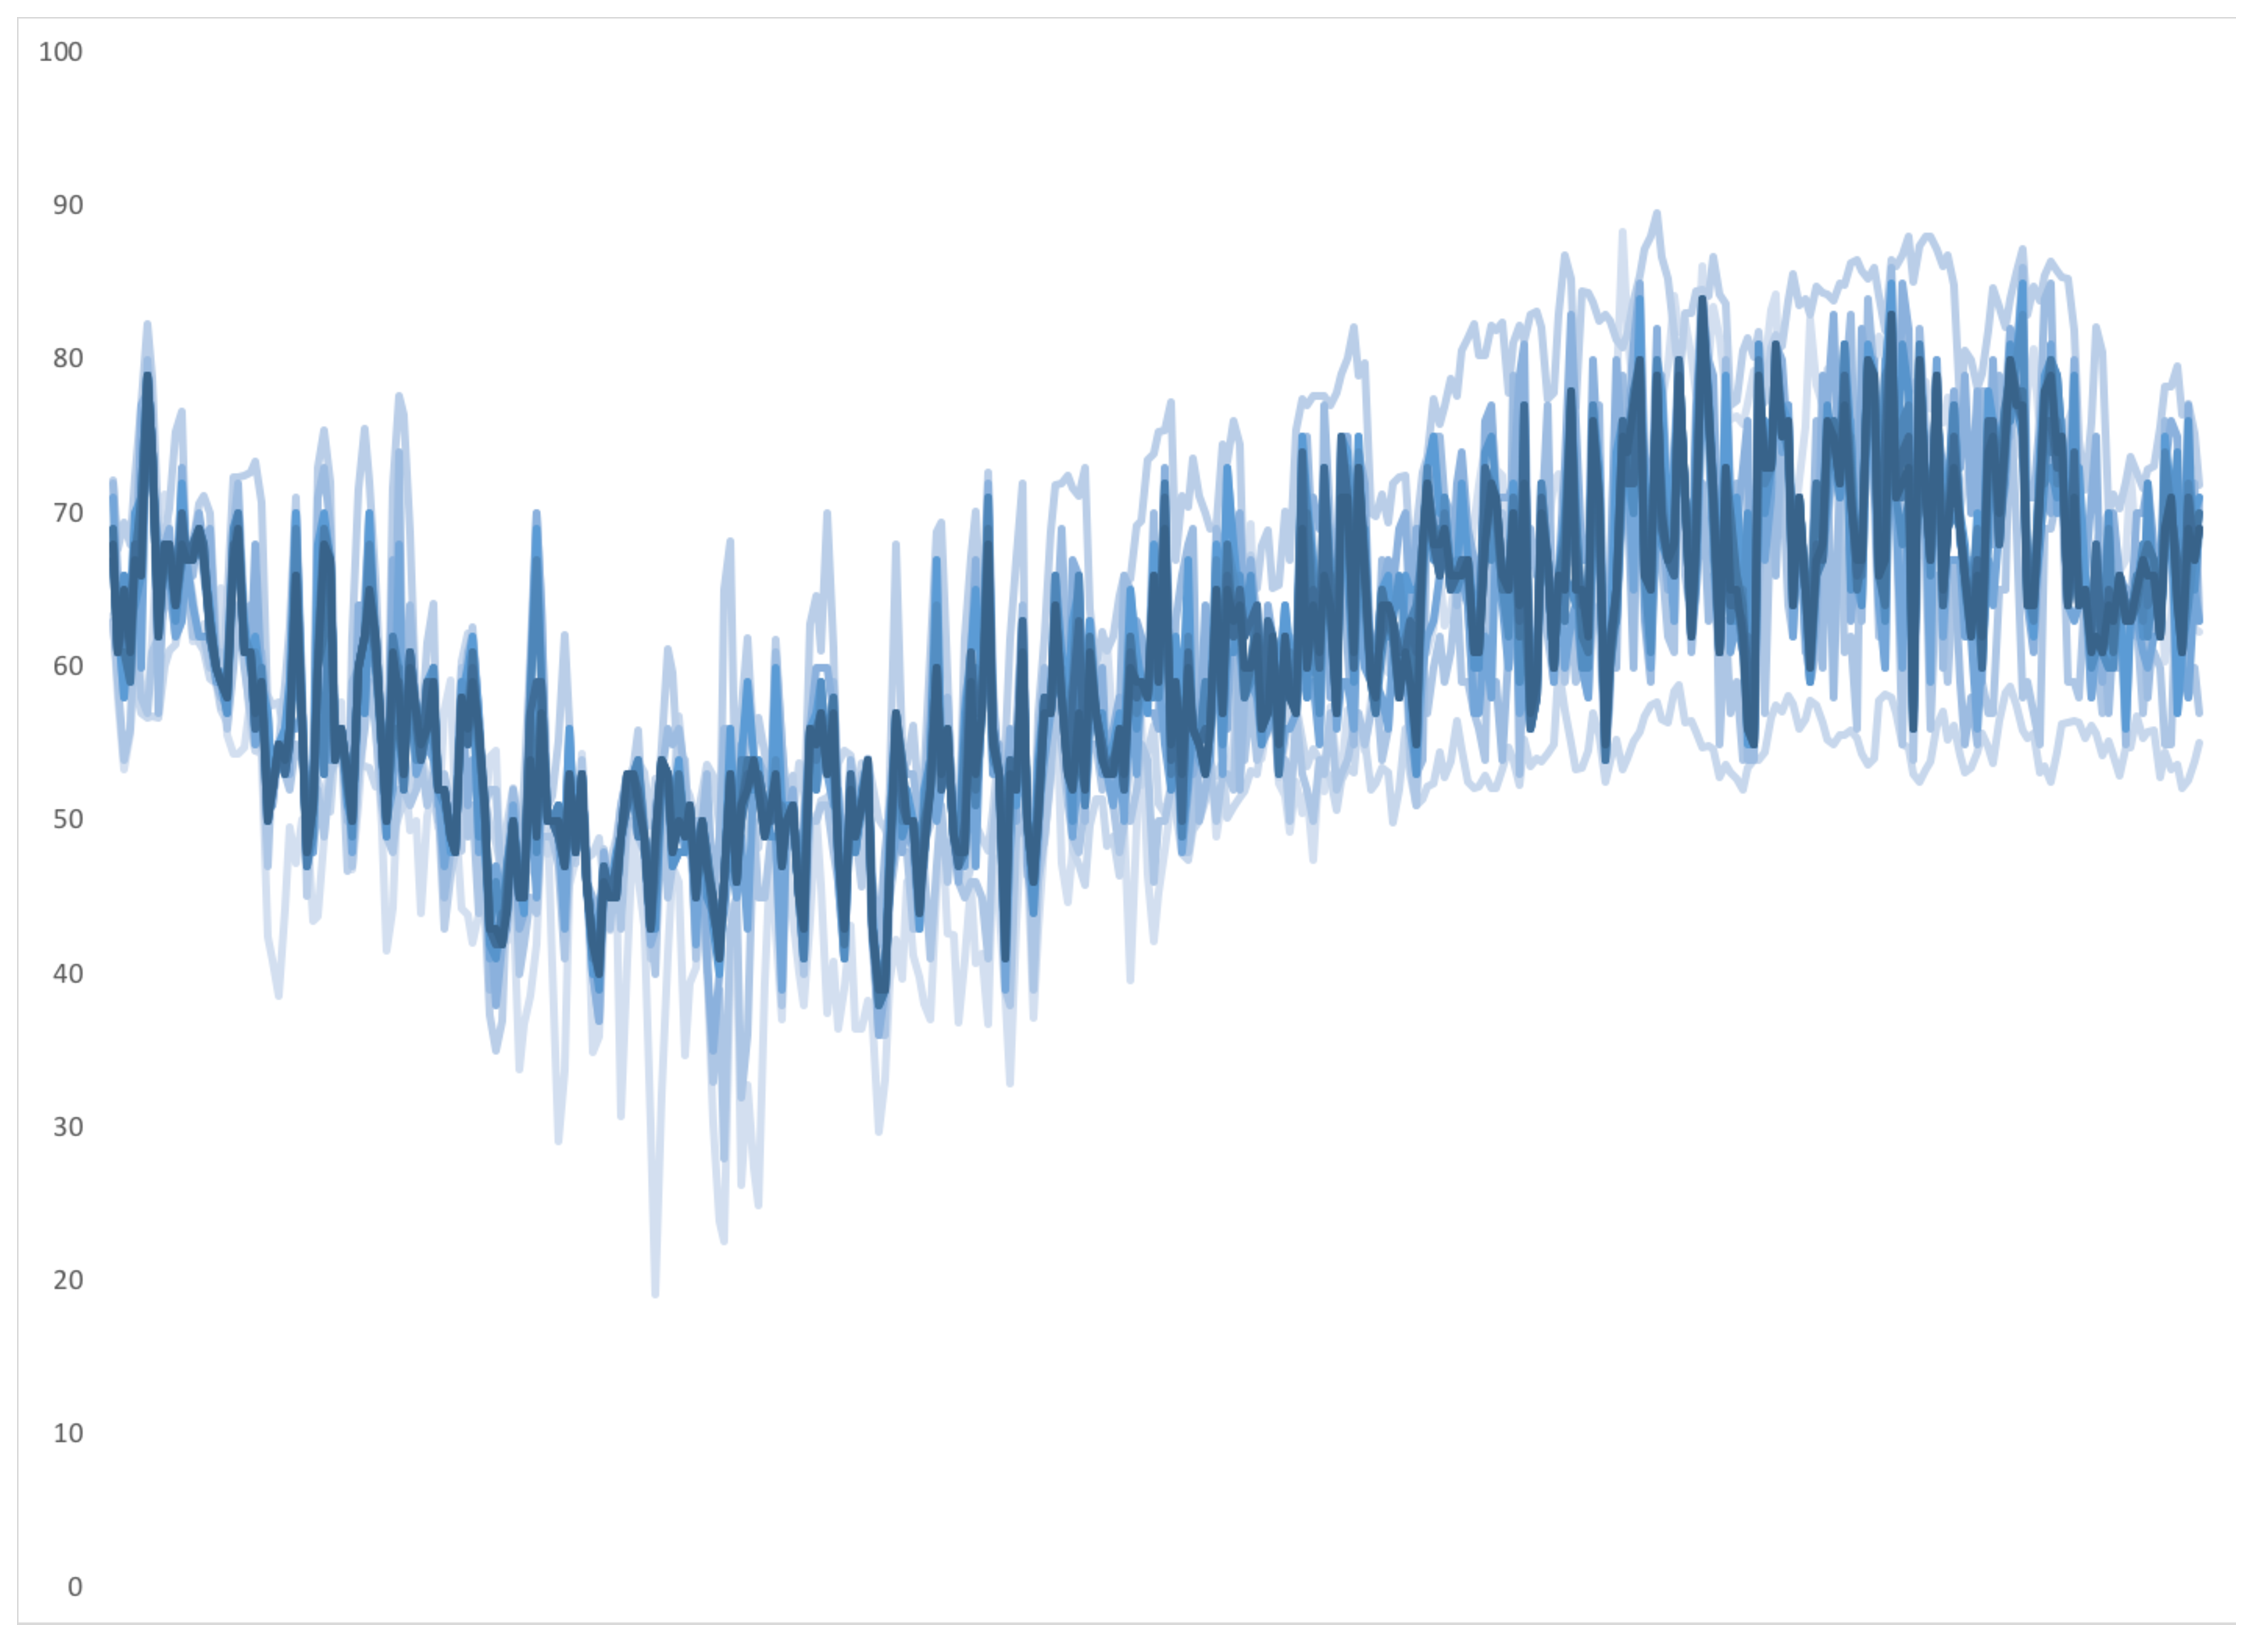
\includegraphics[width=\columnwidth]{images/ensemble}
		\caption{Line ensembles}
	\end{subfigure}%
	~ 
	\begin{subfigure}[t]{.3\columnwidth}
		\centering
		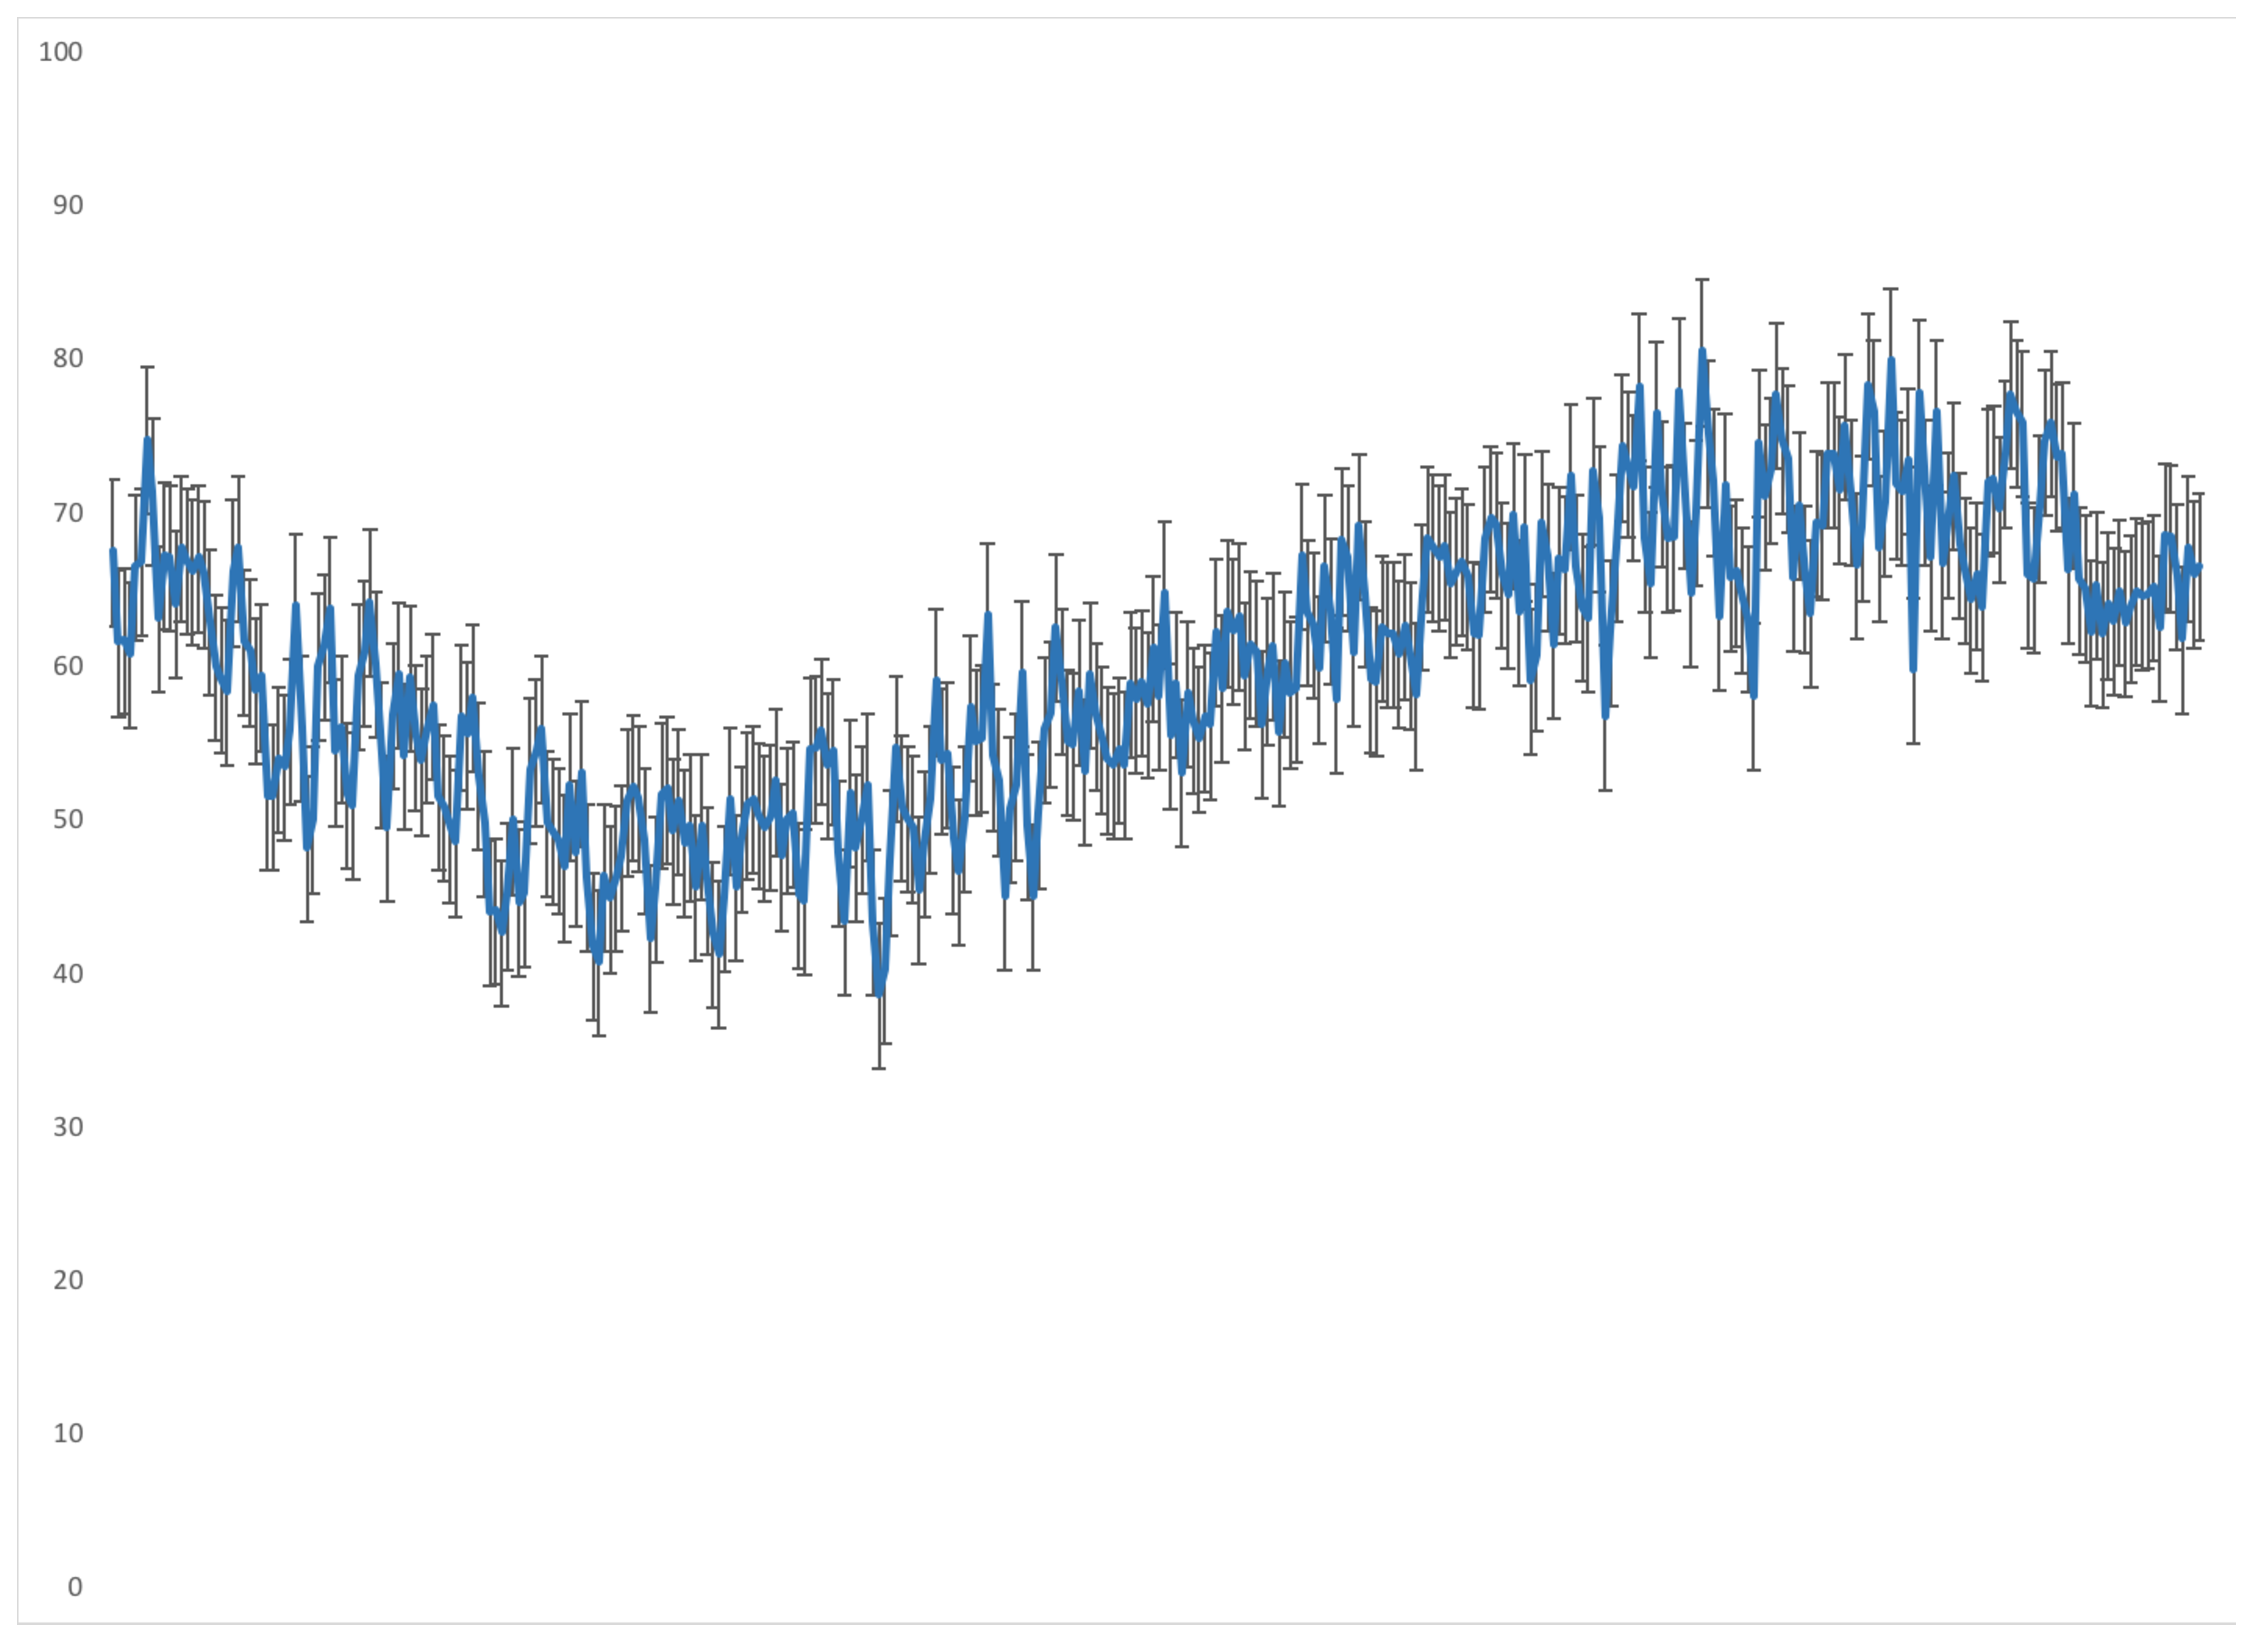
\includegraphics[width=\columnwidth]{images/errorbars}
		\caption{Line with error bars}
	\end{subfigure}
	~ 
	\begin{subfigure}[t]{.3\columnwidth}
		\centering
		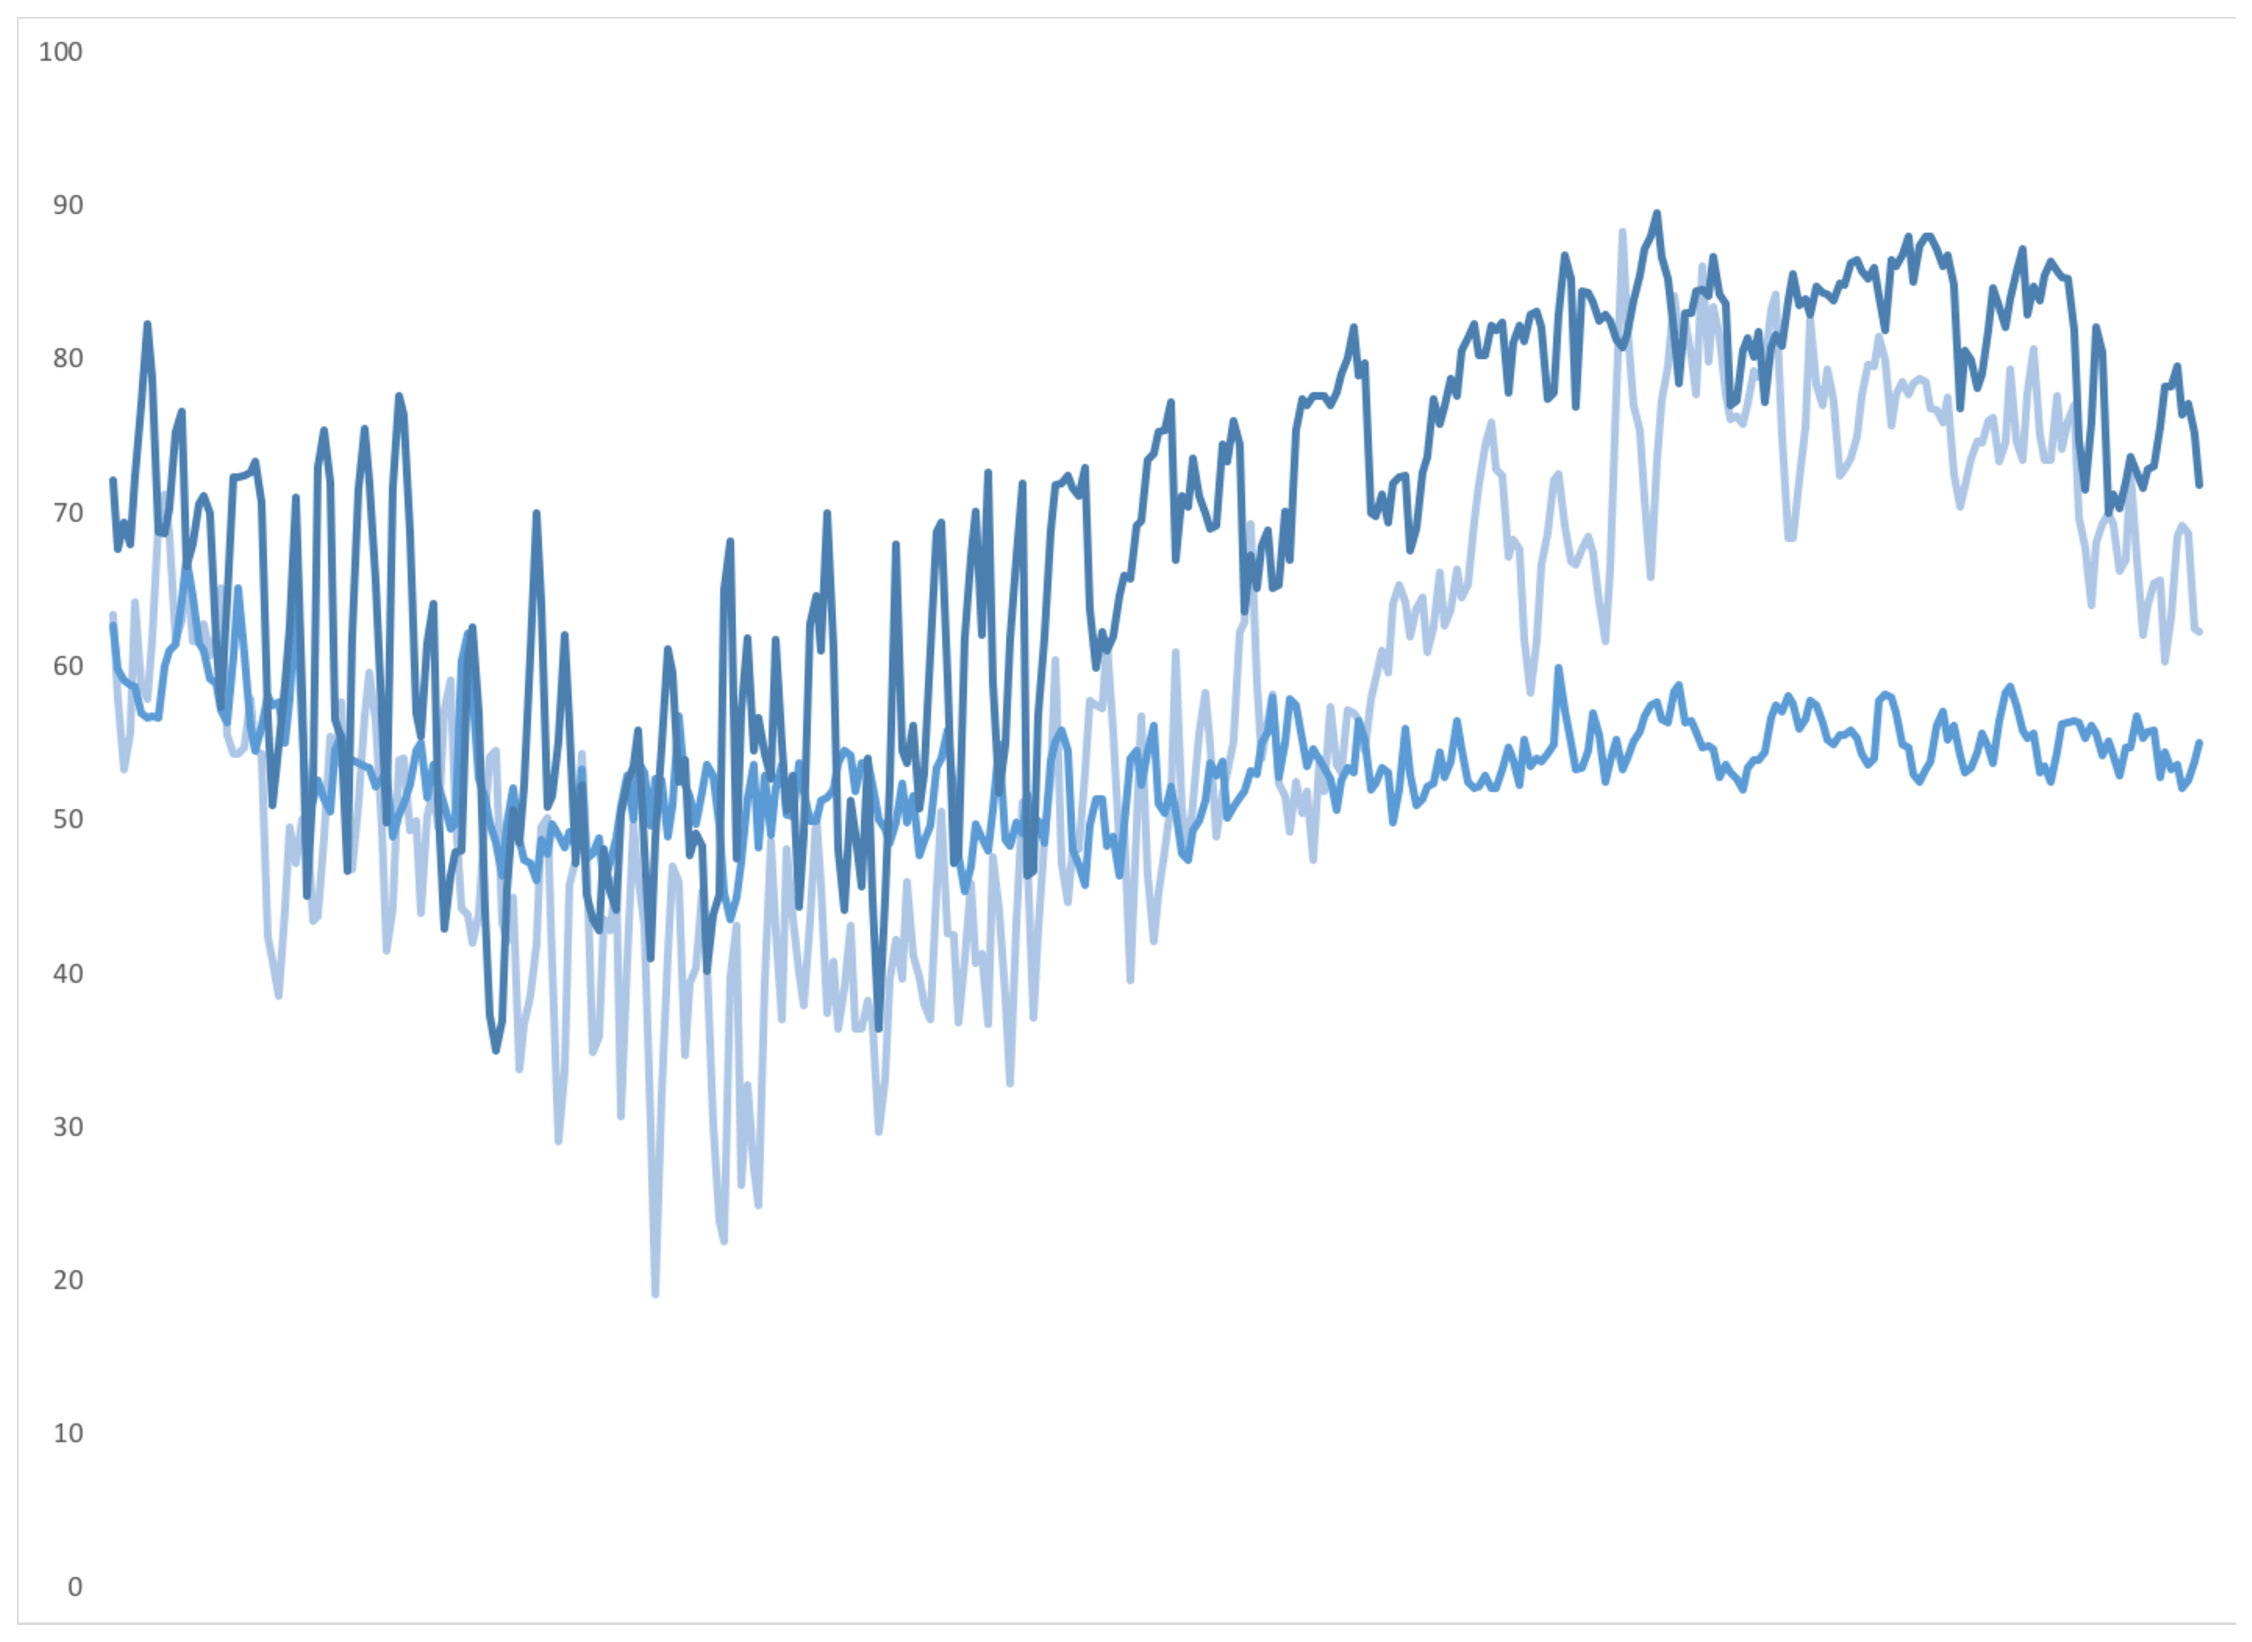
\includegraphics[width=\columnwidth]{images/hops}
		\caption{Hypothetical outcome plots}
	\end{subfigure}
	\caption{We will evaluate visualization techniques for representing uncertainty with time series data. The existed methods include: (a) Line ensembles, (b) error bars, and (c) hypothetical outcome plots~\cite{hullman2015hypothetical}  (an animation that randomly draws from the distribution of possible outcomes.) }
	\label{fig:uncertainty}
\end{figure*}


Communicating uncertainty is one of the greatest challenges we face today.
It impacts many data-driven communities such as climate science~\cite{brodlie2012review,pothkow2011probabilistic,potter2009ensemble,spiegelhalter2011visualizing}, business~\cite{griethe2005visualizing,rodriguez2010toward} and medicine~\cite{han2011varieties,han2011communication,kniss2005statistically,lundstrom2007uncertainty,politi2007communicating,prassni2010uncertainty,spiegelhalter2011visualizing}. 
Visualization has been widely successful in helping people explore, reason, and make judgments with data, and prior work suggests that it may be key for improving comprehension of probability and uncertainty~\cite{correll2014error,brodlie2012review,pothkow2011probabilistic,sanyal2009user,sanyal2010noodles,spiegelhalter2011visualizing}. Researchers have proposed several designs including line ensembles~\cite{potter2009ensemble,sanyal2010noodles}, error bars~\cite{correll2014error}, gradient plots~\cite{correll2014error,han2011communication,jackson2008displaying,tak2014perception} and violin plots~\cite{correll2014error,hintze1998violin,kampstra2008beanplot}. 
More recently, Hullman et al. introduced the hypothetical outcome plot which is an animated chart that randomly draws from the distribution of possible outcomes~\cite{hullman2015hypothetical}. 

One advantage of visualization is that it can make complex or abstract concepts easier to grasp by making them visible. In theory, an effective visual representation can make traditionally difficult problems more concrete and easier to understand. 
In practice, however, nuanced contextual factors heavily impact the effectiveness of visualizations, making the right representation difficult to establish.
While many designs exist, it is not clear whether these methods effective communicate uncertainty and support decision-making in real-world tasks.
Many open questions remain. For instance: \textit{Which visualizations best communicates data with uncertainty}? and \textit{How do
	visualizations impact decision-making?}

In this phase of the project, we will explore and evaluate methods for communicating uncertainty to non-experts.
To identify the best techniques, we will rigorously examine existing methods. 
These include using line ensembles (Figure ~\ref{fig:uncertainty}a), using standard error bars (Figure ~\ref{fig:uncertainty}b), using animation (Figure ~\ref{fig:uncertainty}c), as well as other techniques that leverage visual variables (e.g., scaling the size of visual elements, using color to encode the degree of uncertainty, and using transparency or blurring). 
We plan first to test the designs with a diverse population of study participants via Amazon's Mechanical Turk. 
Once we have some candidate visualizations, we will expand these results by testing real aggregated data with clients in their natural work environments.
Dr. Ottley and her team have extensive experience in evaluating systems.
Here we outline the steps we will take to evaluate the different designs.   

\paragraph{Comparing Designs} 
Our goal here is to determine the most effective visualization design for conveying meaningful information and for facilitating decision-making.  
We will conduct experiments via Amazon's Mechanical Turk using three different evaluation approaches.
\begin{itemize}
	\item[(1)] We will measure speed and accuracy as participants complete standard search and retrieval tasks.
	\item[(2)] Participants will perform decision-making tasks, and we will investigate how each visualization impacts the decisions made.
	\item[(3)] During our experiment, we will conduct additional post-tests using adaptations of standard questionnaires. For instance, we will use the NASA-TLX for subjective measures of workload~\cite{hart1988development}, and the System Usability Scale for measuring perceived usability~\cite{bangor2008empirical}. 
\end{itemize}



\paragraph{Application to Visualization Theory} 
Our proposed work of exploring techniques for communicating uncertainty has applications beyond our problem statement. Visualizing uncertainty is a central challenge in the Information Visualization community with many applications including weather, health, business, and government. Evaluating and potentially developing novel visualization techniques for representing uncertainty will be a signification contribution to these application areas.  

\subsection{Judging Success}
\label{sec:exp}

Ultimately, this project will be successful if we can effectively
protect the privacy of individual data contributors (i.e., a small
privacy budget) concurrently with releasing aggregate data that has
high utility (i.e., low uncertainty).  While theory tells us we cannot
be perfect at one without sacrificing the other, the intention
is to determine how close to that ultimate scenario it is to possible to be.

At the completion of Phase~I, a judgment is required to determine if
further effort towards the above ultimate goal is warranted.
Because that judgment is both a commercial and a technical judgment, we
plan to collaborate with GSI to identify individual potential
customers for the assessment.

One source of information that we will pursue is the International
Poultry Expo, a trade show sponsored by the U.S. Poultry \& Egg Association,
which is held annually in late January.
This meeting is extremely well attended (tens of thousands participate)
and, as such, will serve as fertile ground for helping us assess the
degree to which we have a technical solution that: (1)~provides reasonable
privacy/utility tradeoffs, (2)~effectively communicates those tradeoff
choices to farmers, and (3)~can be offered in a way that farmers are
likely to participate.

The meeting is timely, in that it happens towards the end of the
Phase~I schedule period. During the meeting, we will solicit
participants to assist us in evaluating our technical solutions.
This is the primary method by which
we will judge whether or not we have been successful
in the Phase~I effort.

